% tikz diagram with a 3d perspective illustrating how web3
% and metamask can interactive with IPFS and Solidity

\documentclass{article}
\usepackage{tikz}

\usepackage{verbatim}
\usepackage[active,tightpage]{preview}
\PreviewEnvironment{tikzpicture}
\setlength\PreviewBorder{5pt}%

\usetikzlibrary{positioning}

\newcommand{\yslant}{0.5}
\newcommand{\xslant}{-0.6}
\begin{document}
\begin{tikzpicture}[scale=1.1,every node/.style={minimum size=1cm},on grid]

	% Software level
	\begin{scope}[
		yshift=-120,
		every node/.append style={yslant=\yslant,xslant=\xslant},
		yslant=\yslant,xslant=\xslant
	] 
		% The lower frame:
		\draw[black, dashed, thick] (-1.3,0) rectangle (8.2,4.8); 
		% Agents:
		\draw[fill=red]  
			(7.5,2) circle (.1) % .pdf file
			(5,2) circle (.1) % .ps file
			(2,2) circle (.1) % .dvi file
			(-0.5,2) circle (.1); % .tex file
		% Flows:
		\draw[-latex,ultra thick,shorten <=5pt,shorten >=5pt] 
			(-0.5,2) to[out=0,in=-180] (2,2); % latex
		\draw[-latex,ultra thick,shorten <=5pt,shorten >=5pt] 
			(2,2) to[out=0,in=-180] (5,2); % dvi2ps
		\draw[latex-latex,ultra thick,shorten <=5pt,shorten >=5pt] 
			(5,2) to[out=0,in=-180] (7.5,2); % ps2pdf, pdf2ps
		\draw[-latex,ultra thick,shorten <=5pt,shorten >=5pt] 
			(-0.5,2) to[out=90,in=-180] (3.5,3.8) to[out=0,in=90] (7.5,2); % pdflatex
		\draw[-latex,ultra thick,shorten <=5pt,shorten >=5pt] 
			(2,2) to[out=90,in=-180] (2.7,3.0) to[out=0,in=-180] (6.7,3.0) to[out=0,in=135] (7.5,2); % ps2pdfm
		 % Labels:
		\fill[black]
			(1.0,2) node[above=-3pt, scale=0.9] {\textsf{\bfseries file}}			
			(3.5,2) node[above=-5pt, scale=0.9] {\textsf{\bfseries hash}}
			(6.25,2) node[above=-5pt, scale=0.9] {\textsf{\bfseries interacts}}

			(3.5,3.8) node[xshift=2ex,below=-5pt, scale=0.9] {\textsf{\bfseries logic contained in}}
			(4.3,3.0) node[xshift=2ex,below=-5pt, scale=0.9] {\textsf{\bfseries complements}}
			(1.3,0.1) node[above=-2pt, scale=1.1] {\textbf{Blockchain/Ethereum Level}}
			(-0.5,2) node[below,scale=.9]{\textsf{\bfseries Dapp} }
			(2,2) node[below,scale=.9]{\textsf{\bfseries IPFS}}
			(5,2) node[below,scale=.9]{\textsf{\bfseries Metamask}}
			(7.5,2) node[below,scale=.9]{\textsf{\bfseries Solidity}};	
	\end{scope}
	
	% vertical lines for linking agents on the 2 levels
	\draw[thick](6.3,5.1) to (6.3,0.9);
	\draw[thick](3.8,4) to (3.8,-0.32);
	\draw[thick](0.8,2.4) to (.8,-1.8);
	\draw[thick](-1.70,1.02) to (-1.70,-3);
	
	% User level
	\begin{scope}[
		yshift=0,
		every node/.append style={yslant=\yslant,xslant=\xslant},
		yslant=\yslant,xslant=\xslant
	]
		% The upper frame:
		\fill[white,fill opacity=.70] (-3.1,0) rectangle (9.9,6); % Opacity
		\draw[black, dashed, thick] (-3.1,0) rectangle (9.9,6); 
		 % Agents:
		\draw [fill=red]
			(7.5,2) circle (.1) % .pdf file
			(5,2) circle (.1) % .ps
			(2,2) circle (.1) % .dvi
			(-0.5,2) circle (.1); % .tex file

		% the icons
		\node[anchor=south,inner sep=0,xshift=-20pt,yshift=10pt,fill=white] at (-0.5,2)
			{
\includegraphics[width=2.5cm]{truffle.png}};
		\node[anchor=south,inner sep=0,xshift=0pt,yshift=8pt] at (2,2)
			{
\includegraphics[width=2.5cm]{ipfs-logo.png}};
		\node[anchor=south,inner sep=0,xshift=-5pt,yshift=8pt] at (5,2)
			{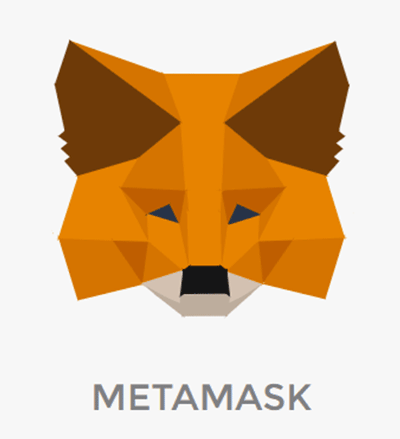
\includegraphics[width=3.0cm]{metamask.png}};
		\node[anchor=south,inner sep=0,xshift=20pt,yshift=8pt] at (7.5,2)
			{
\includegraphics[width=3.5cm]{ethereum.png}};

		\fill[black]
			(7.5,2) node[below right,,xshift=-20pt,yshift=-5pt,scale=.9,text width=2.5cm,align=left,fill=white]
				{\textsf{\bfseries \mbox{Smart Contracts}}\\ \textsf{\bfseries IPFS Hashes}
				\\ \textsf{\bfseries Authentication}}
			(-2.5,5.5) node[anchor=west,inner sep=0, scale=1.1] {\textbf{User level}}
			(5.1,1.9) node[below right,xshift=-20pt,scale=.9,text width=2cm,align=left,fill=white]
				{\textsf{\bfseries Transactions}\\ \textsf{\bfseries Ethereum Browser} }
			(1.9,1.9) node[below right,xshift=-10pt,scale=.9,text width=2cm,align=left,fill=white]
				{\textsf{\bfseries File Storage}\\ \textsf{\bfseries Peer to Peer}}
			(-0.5,2) node[below right,xshift=-20pt,yshift=-5pt,scale=.9,text width=2.5cm,align=left,fill=white]
				{\textsf{\bfseries Drizzle}\\ \textsf{\bfseries React}\\
					\textsf{\bfseries Truffle}} 
		;
	\end{scope} 
\end{tikzpicture}
\end{document}
